
% This LaTeX was auto-generated from MATLAB code.
% To make changes, update the MATLAB code and republish this document.

\documentclass{article}
\usepackage{graphicx}
\usepackage{color}

\sloppy
\definecolor{lightgray}{gray}{0.5}
\setlength{\parindent}{0pt}

\begin{document}

    
    
\section*{Grand Canyon Problem}


\subsection*{Contents}

\begin{itemize}
\setlength{\itemsep}{-1ex}
   \item Determining accleration
   \item Numerical No Drag
   \item Numerical With Drag
   \item Functions
\end{itemize}
\begin{verbatim}
%Johnathan Corbin
%Spring 2019
\end{verbatim}


\subsection*{Determining accleration}

\begin{verbatim}
clear, clc

syms omega x y z xv yv zv xa ya za phi rho cD A
w = [0; omega*cos(phi); omega*sin(phi)];
rOP = [0; 0; 6380];
rPQ = [x; y; z];
aQP = [xa; ya; za];
vQP = [xv; yv; zv];
aP = cross(w, cross(w, rOP));

aQ = aP + aQP + cross(w, cross(w, rPQ)) + 2*cross(w, vQP);
\end{verbatim}


\subsection*{Numerical No Drag}

\begin{verbatim}
%global A CD rOP m rho Omega u d
global d A CD rOP m rho Omega u

A = pi * .05^2; %Frontal area of the sphere
CD = 0;
rOP = (6378 + 2) * 1000; %Position vector from center of earth to cliff
m = 1; %Mass of the rock.
rho = 1.225; %Density of air at sea level
Omega = [0; (7.292*10^-5)*cos(34 * pi / 180); (7.292*10^-5)*sin(34 * pi / 180)];
u = 398600 * (1000^3); %Gravitation coefficient
d = 1500;

fname = 'Canyon'; % Setting name of the .m file for the state variable time derivatives

initial_conditions = [0; 0; 0; 0; 0; 0];

Opt = odeset('Events', @GC_Event);
[time, y, te, ye, ie] = ode45(@Canyon, [0, 1e6], initial_conditions, Opt);
figure(1)
plot(time, y(:,1), 'k')
hold on
plot(time, y(:,2), '--k')
title('Rock Falling with No Drag')
legend('X-Position','Y-Position', 'Location', 'best')
xlabel('Time (sec)')
ylabel('Meters')
\end{verbatim}

        \color{lightgray} \begin{verbatim}Warning: The value of local variables may have been changed to match the
globals.  Future versions of MATLAB will require that you declare a variable to
be global before you use that variable. 
Warning: The value of local variables may have been changed to match the
globals.  Future versions of MATLAB will require that you declare a variable to
be global before you use that variable. 
Warning: The value of local variables may have been changed to match the
globals.  Future versions of MATLAB will require that you declare a variable to
be global before you use that variable. 
\end{verbatim} \color{black}
    
\includegraphics [width=4in]{Code_01.eps}


\subsection*{Numerical With Drag}

\begin{verbatim}
CD = 0.42;
Opt = odeset('Events', @GC_Event);
[time, y, te, ye, ie] = ode45(@Canyon, [0, 1e6], initial_conditions, Opt);
figure(2)
plot(time, y(:,1), 'k')
hold on
plot(time, y(:,2), '--k')
title('Rock Falling with Drag')
legend('X-Position','Y-Position', 'Location', 'best')
xlabel('Time (sec)')
ylabel('Meters')
\end{verbatim}


\subsection*{Functions}

\begin{verbatim}
function dydt = Canyon(t, y)

global A CD rOP m rho Omega u

dydt = zeros(size(y));

F_g = -(u*m/(rOP + y(3))^2)*[0; 0; 1];

F_D = -(1/2) * rho * CD * A * sqrt(y(4)^2 + y(5)^2 + y(6)^2) * [y(4); y(5); y(6)];

rOQ = (rOP) * [0; 0; 1] + [y(1); y(2); y(3)];

acceleration = (F_g + F_D - m * (cross(Omega, cross(Omega, rOQ)) + 2*cross(Omega,[y(4);y(5);y(6)])))/m;

dydt(1) = y(4);
dydt(2) = y(5);
dydt(3) = y(6);
dydt(4) = acceleration(1);
dydt(5) = acceleration(2);
dydt(6) = acceleration(3);
end

function [value,isterminal,direction] = GC_Event(time,y)
% The second arguement of this function is the system state vector being
% integrated by ODE45
global d
%Event funtion to stop integration when rock hit -1500[m]
%if y(3) > -1500 %If rock is higher than -1500[m]
if y(3) > -d %If rock is higher than -1500[m]
 value = 1; %Keep going
else %If not
 value = 0; %Then stop
end
isterminal = 1; %Terminate integration when condtion met
direction = 0; %Direction doesn't matter
end
\end{verbatim}



\end{document}
    
